\section{Tinjauan Pustaka}

Kluster Merupakan sebuah teknologi yang dibuat sebagai upaya untuk mendapatkan kemampuan komputasi besar dengan harga murah. hal ini dilakukan dengan cara menghubungkan komputer, baik \textit{standalone}, terdistribusi, maupun paralel, dengan tujuan untuk membagi pekerjaan yang sebelumnya hanya dapat dilakukan oleh satu komputer saja secara bersamaan \cite{cloud_computing}. Untuk membagi tugas didalam setiap node, digunakan teknologi yang bernama Kontainerisasi.

\vspace{0.2cm}
\noindent Kontainerisasi memberikan kemampuan kepada pengembang untuk menciptakan aplikasi port-able \cite{containers}. menggunakan kontainerisasi, sebuah node dapat menjalankan berbagai macam tugas secara bersamaan, tanpa perlu mengkhawatirkan terjadinya konflik antar proses mengenai sumber daya yang ada. Seperti versi program yang berbeda, pustaka program yang tidak dapat ada secara bersamaan, dan kebutuhan akan integrasi kuat antar program di dalam kontainer. Selain itu, terdapat pula faktor keamanan dimana ketika sebuah kontainer terkontaminasi atau terkena serangan eksternal, tidak akan terjadi kerusakan pada kontainer lain karena isolasi yang diberikan oleh teknologi ini.

\vspace{0.2cm}
\noindent Penggunaan Raspberry Pi dalam server sederhana dan perangkat keras komputer juga meningkat seiring dengan berjalannya waktu. hal ini disebabkan oleh semakin tingginya angka pengembang aplikasi yang membutuhkan perangkat IoT dan lingkungan pengembangan murah untuk didapatkan dan/atau untuk digunakan sebagai sarana pembelajaran \cite{raspi_market}.

\subsection{Kubernetes}

Kubernetes memberikan sebuah platform open source portabel yang dapat diperluas untuk mengelola beban kerja dan layanan dalam container dalam bentuk orkestrasi, yang memfasilitasi konfigurasi deklaratif dan otomatisasi \cite{kubernetes_overview}. Didalamnya, terdapat Kluster, yang terdiri dari sekumpulan mesin pekerja, yang disebut node, yang menjalankan aplikasi dalam container. Setiap cluster memiliki setidaknya satu node pekerja \cite{kubernetes_components}. Node sendiri adalah sebuah perangkat keras maupun virtual yang bertugas menjalankan program didalam kontainer yang disebut Pods yang diluncurkan kedalam kluster yang diatur oleh sebuah \textit{controlplane} \cite{kubernetes_nodes}. Komponen komponen tersebut bersinergi dan bekerja sama dalam membentuk lingkungan perangkat lunak yang dapat terskala dan tumbuh secara horizontal. Sehingga dapat memberikan peluang baru bagi pengembang aplikasi dan administrator untuk merubah daya komputasi sesuai kebutuhan aplikasi pada saat tertentu dengan mudah dan mempermudah implementasi \textit{redundancy}.\\
\begin{figure}[htb!]
    \centering
    \begin{tabular}{ @{} r @{} }
        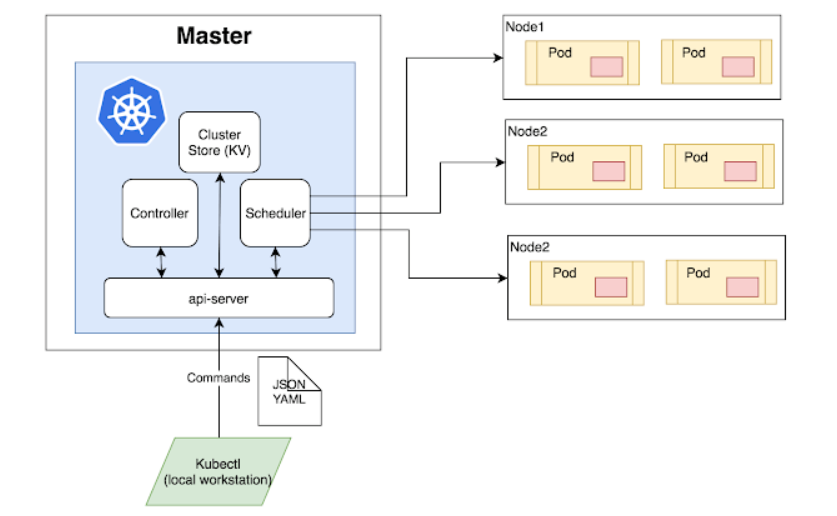
\includegraphics[scale=0.7]{pictures/k8s_diagram.png}\\
        \imagesource{https://www.eternalsoftsolutions.com}
    \end{tabular}
    \caption{Struktur Kubernetes (K8s)}
\end{figure}
\FloatBarrier

\subsection{Raspberry Pi}

Raspberry Pi adalah komputer kecil menggunakan arsitektur ARM murah yang berfungsi seperti komputer pada umumnya \cite{raspi}. Perangkat keras ini memberikan akses komputasi murah untuk menciptakan perangkat-perangkat lain seperti Internet of Things (IoT), Personal Computer (PC), dan Server. Dan karena mudahnya mendapatkan perangkat dalam jumlah yang besar, maka Raspberry Pi juga dapat digunakan sebagai node untuk dihubungkan menggunakan Kubernetes dengan K3s.
\begin{figure}[htb!]
    \centering
    \begin{tabular}{ @{} r @{} }
        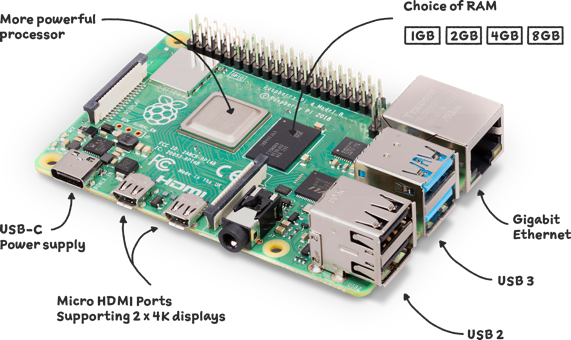
\includegraphics[scale=0.4]{pictures/raspi.png}\\
        \imagesource{https://www.raspberrypi.com/}
    \end{tabular}
    \caption{Komponen Raspberry Pi 4B}
\end{figure}
\FloatBarrier

\subsection{K3s}

K3s merupakan salah satu distribusi Kubernetes tersertifikasi dengan ketersediaan tinggi yang dirancang untuk beban kerja produksi di lokasi terpencil yang tidak diawasi, terbatas sumber daya, atau di dalam peralatan IoT \cite{k3s}. Portabilitas, ketersediaan, dan keringanan yang dimiliki oleh K3s didapatkan dengan memanfaatkan enkapsulasi seluruh komponen nya dalam satu proses. Yang hanya membutuhkan setidaknya 1vCPU dan 512MB RAM \cite{k3s_mk8s}. minimnya penggunaan sumber daya juga menjadi alasan utama pemilihan K3s jika dibandingkan dengan teknologi serupa seperti mK8s (MicroK8s) \cite{k3s_mk8s}. Dan karena enkapsulasi itu pula, tidak dibutuhkan pemasangan \textit{Docker Engine} secara terpisah didalam sistem yang menjalankan K3s.\\
\begin{figure}[htb!]
    \centering
    \begin{tabular}{ @{} r @{} }
        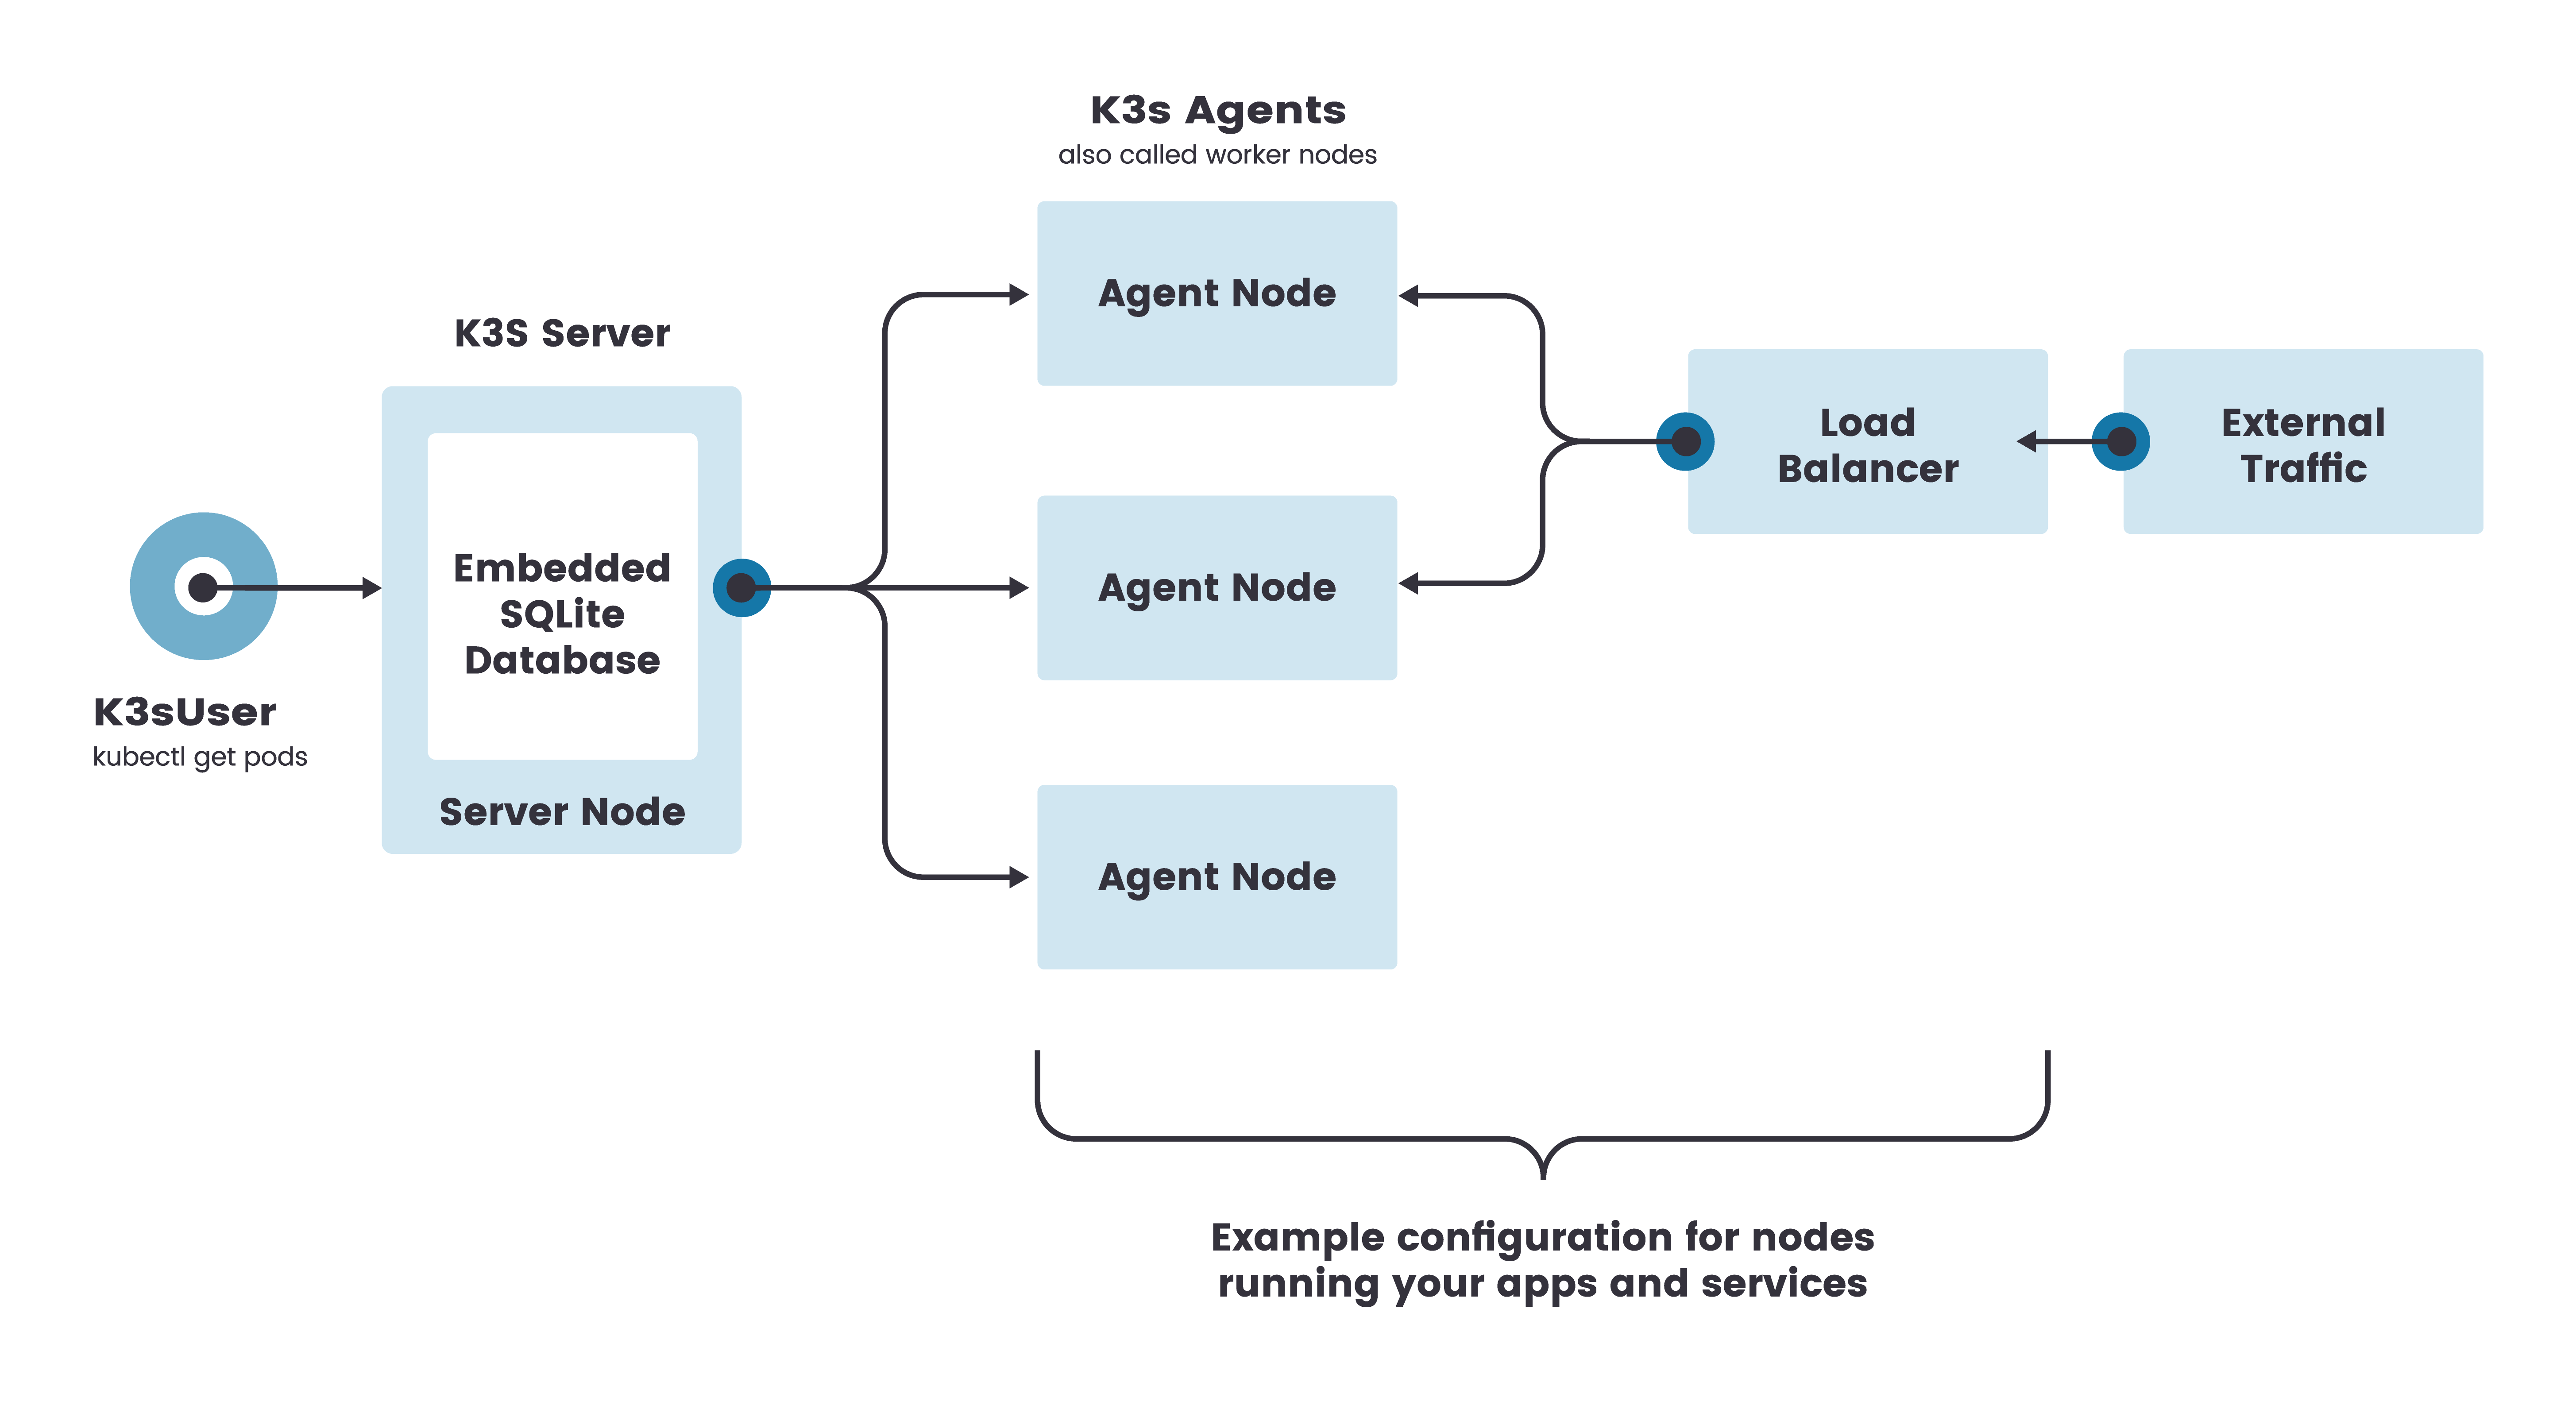
\includegraphics[scale=0.28]{pictures/k3s_diagram.png}\\
        \imagesource{https://nimblehq.co}
    \end{tabular}
    \caption{Struktur K3s}
\end{figure}
\FloatBarrier

\subsection{Ansible}

Ansible memiliki kemampuan untuk menghubungkan dan mempermudah proses pengaturan dan perawatan sistem pada saat peluncuran aplikasi. Karena Ansible mampu melakukan konfigurasi sistem, peluncuran perangkat lunak, dan mampu melakukan orkes-trasi kegiatan teknologi seperti \textit{Circular Integration/Circular Deployment} (CI/CD) \cite{ansible_docs}. menggunakan Ansible, pengaturan berulang yang harus dilakukan untuk setiap Node Rapsberry-Pi dapat di otomatisasi sehingga dapat mengurangi \textit{human error} dan meningkatkan efektifitas waktu.\\
\begin{figure}[htb!]
    \centering
    \begin{tabular}{ @{} r @{} }
        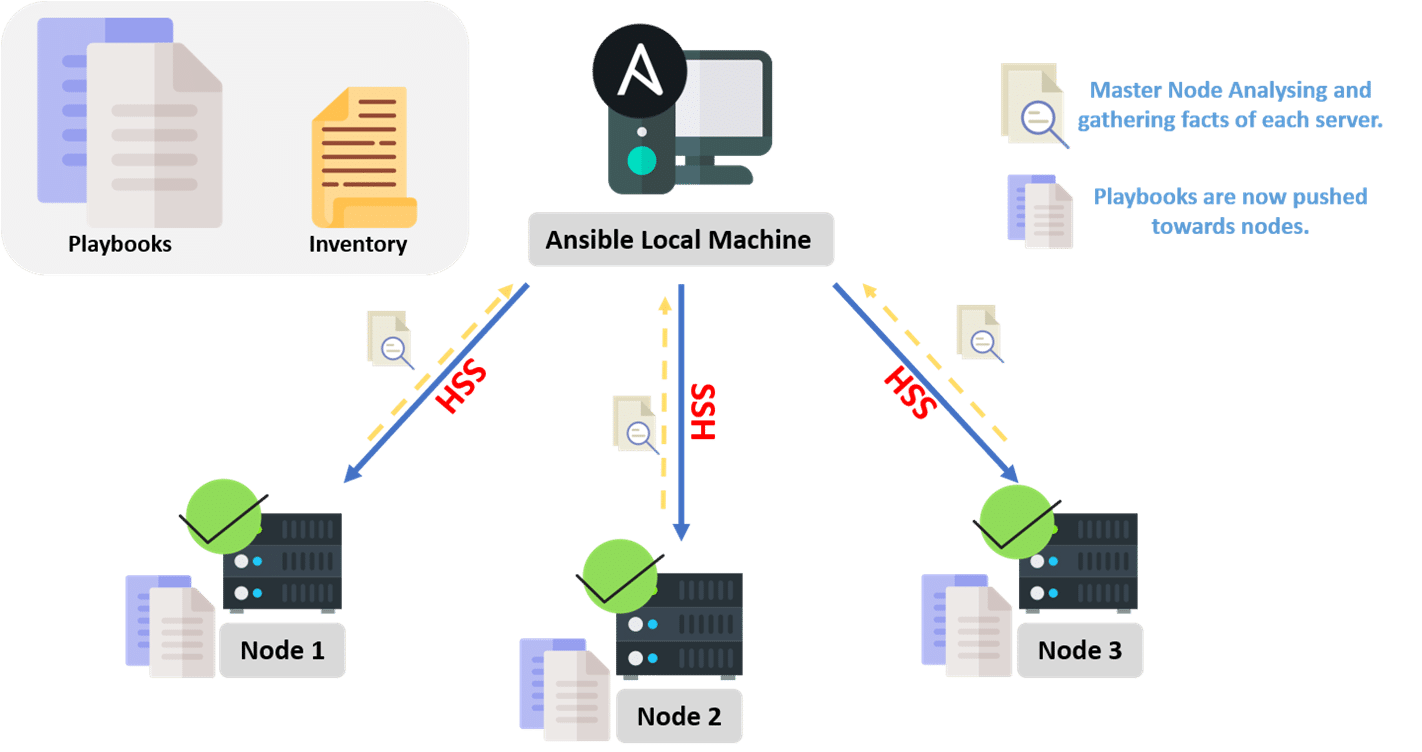
\includegraphics[scale=0.25]{pictures/ansible_node.png}\\
        \imagesource{https://intellipaat.com}
    \end{tabular}
    \caption{Koneksi Ansible menuju Node menggunakan SSH}
\end{figure}
\FloatBarrier
